

\clearpage
\subsection{The Shields merchant}
\label{sec:appendix:moj:shields}

A Viking shield-maker was called a skjaldarsmithr. Shields had to be light so that they could be carried easily into battle but also strong so that they wouldn't split when struck by a sword.

\begin{display}{The shields stall}
	\label{fig:appendix:moj:places:shields:stall}
	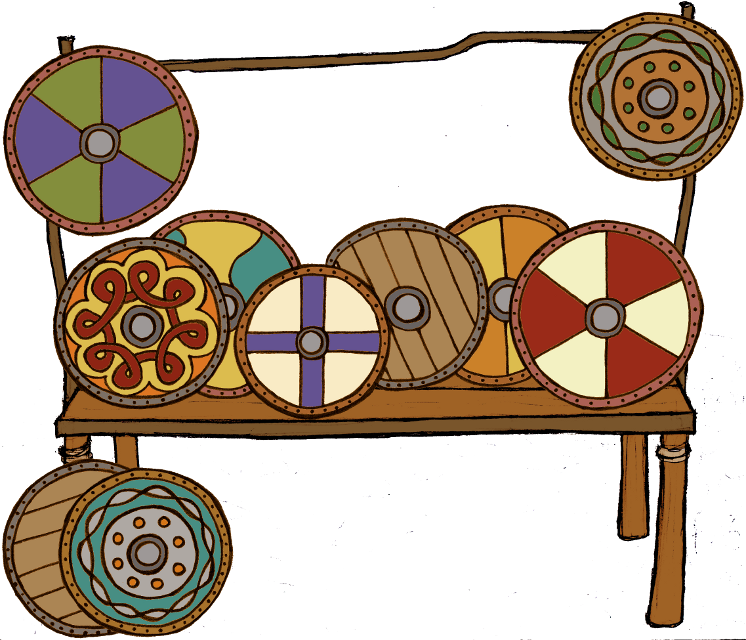
\includegraphics[width=0.65\columnwidth]{img/Jorvik/places/shields stall}
\end{display}

\begin{display}{The shields stall with a background and a merchant}
	\label{fig:appendix:moj:places:shields}
	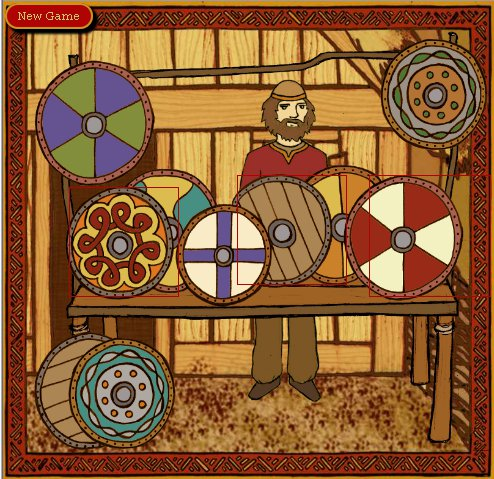
\includegraphics[width=0.65\columnwidth]{img/Jorvik/places/shields}
\end{display}
\clearpage


\begin{table}[ht!]
	\centering
	\begin{tabular}{ p{3cm} c }\toprule
		\textbf{Name:} & \multirow{5}{*}{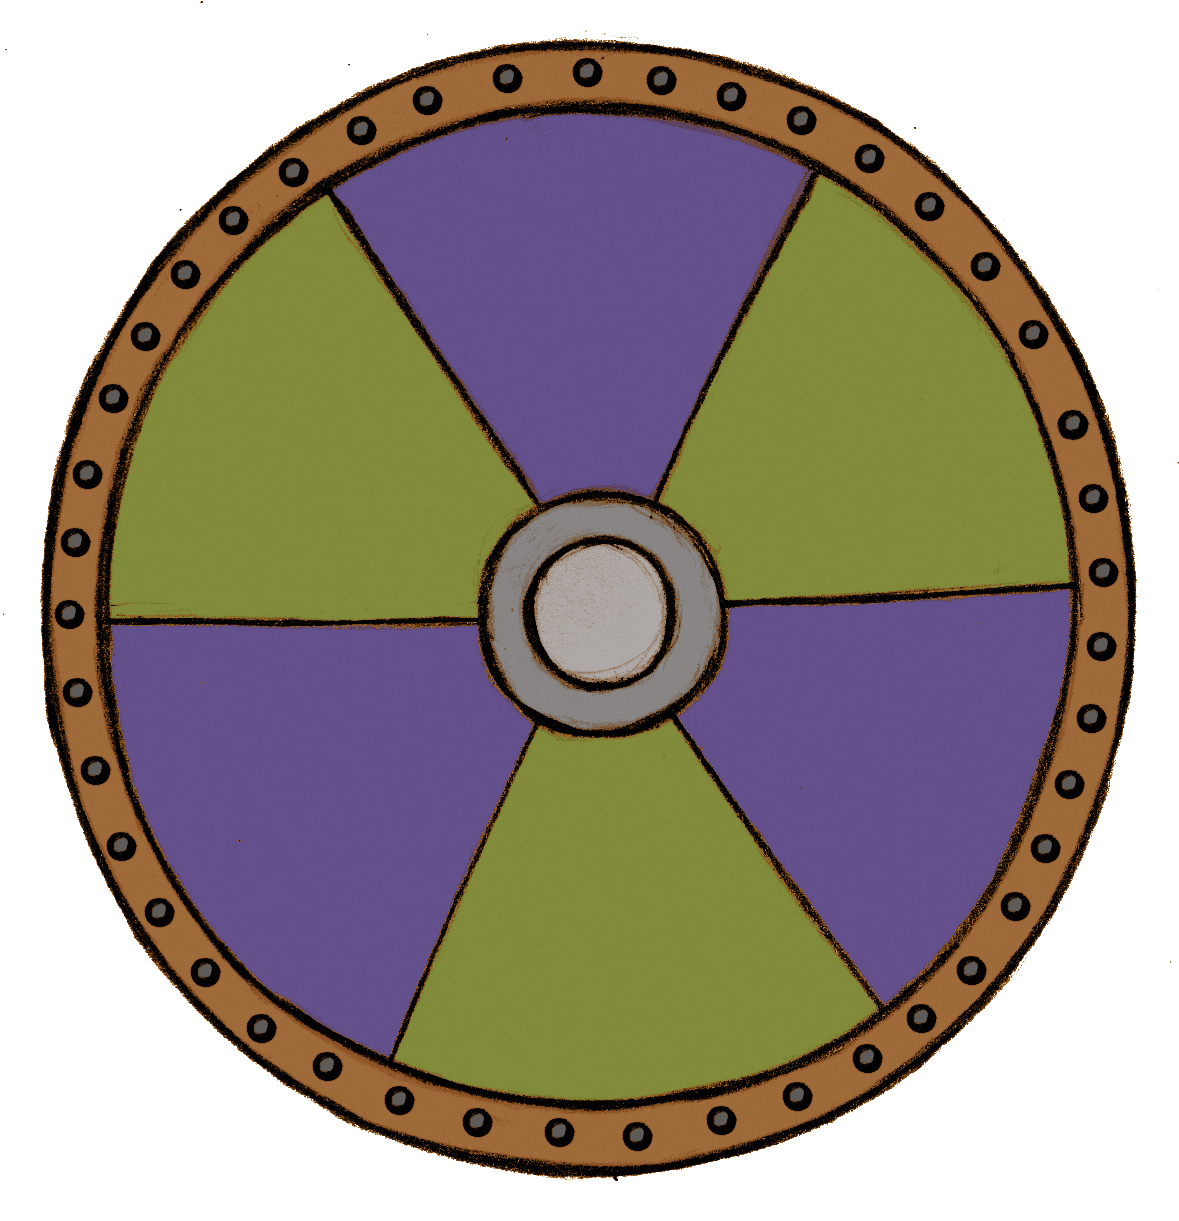
\includegraphics[height=30mm]{img/Jorvik/objects/shields/painted shield}}\\
		Painted Shield & \\ 
		\textbf{Price:} & \\
		37.93 Silver & \\ 
		\textbf{Description:} & \\
		\multicolumn{2}{p{12cm}}{An old Norwegian law dictated that shields should be painted in red and white, though shields have been found in other colours.}\\
		\bottomrule
	\end{tabular}
\end{table}

\begin{table}[ht!]
	\centering
	\begin{tabular}{ p{3cm} c }\toprule
		\textbf{Name:} & \multirow{5}{*}{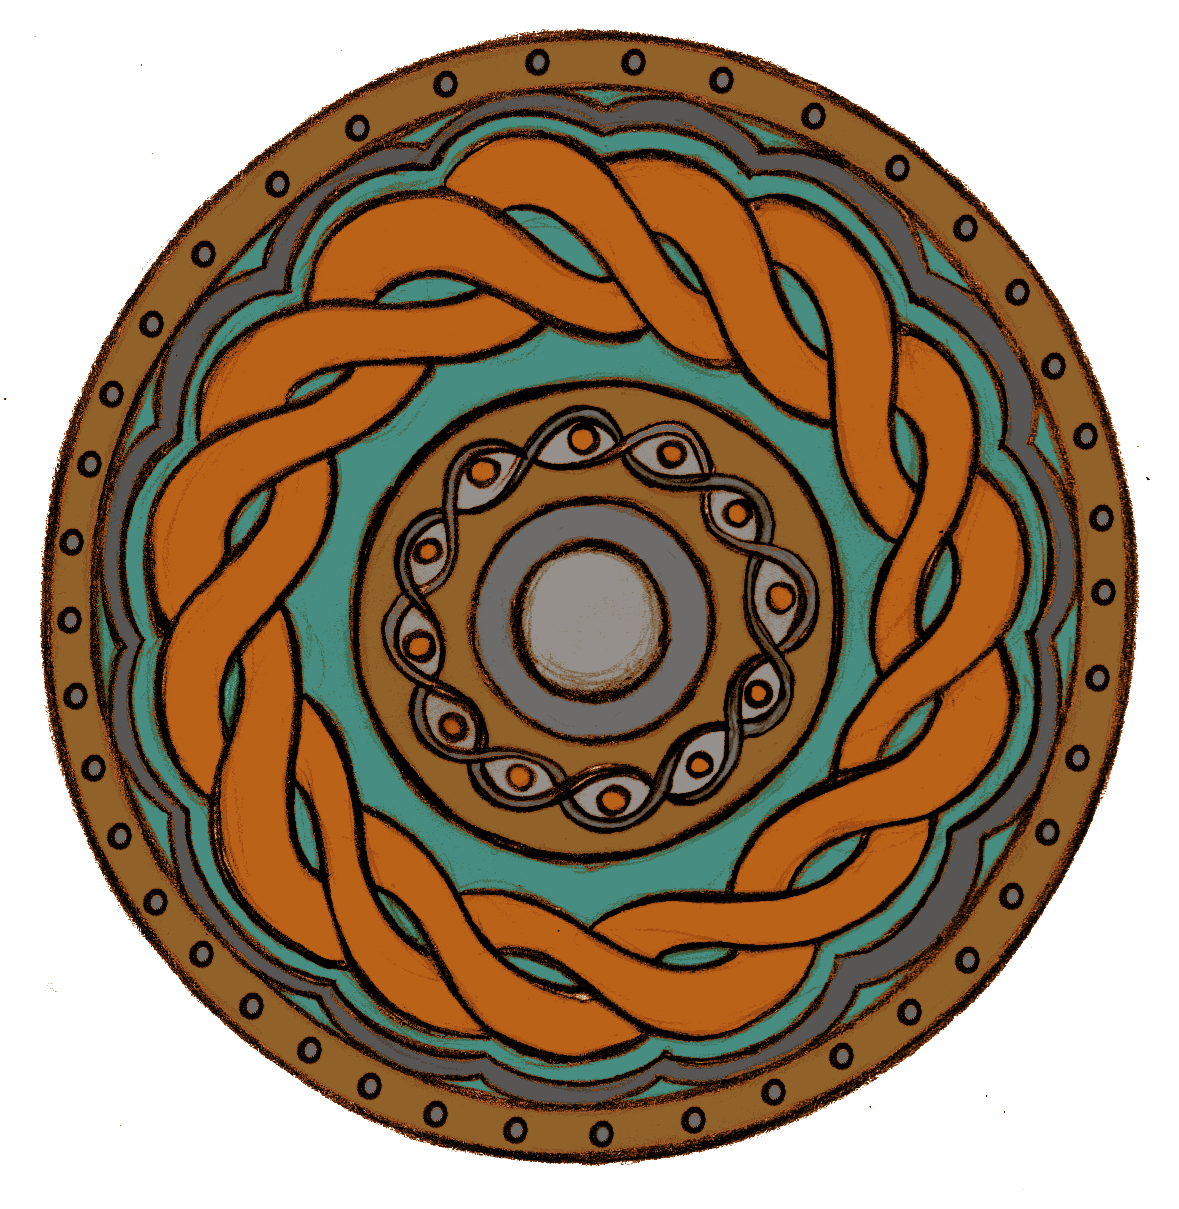
\includegraphics[height=30mm]{img/Jorvik/objects/shields/decorated shield}}\\
		Decorated Shield & \\ 
		\textbf{Price:} & \\
		44.11 Silver & \\ 
		\textbf{Description:} & \\
		\multicolumn{2}{p{12cm}}{Decorated shields were sometimes given as gifts. They could be carved with scenes from Norse myths and be adorned with gold and jewels.}\\
		\bottomrule
	\end{tabular}
\end{table}

\begin{table}[ht!]
	\centering
	\begin{tabular}{ p{3cm} c }\toprule
		\textbf{Name:} & \multirow{5}{*}{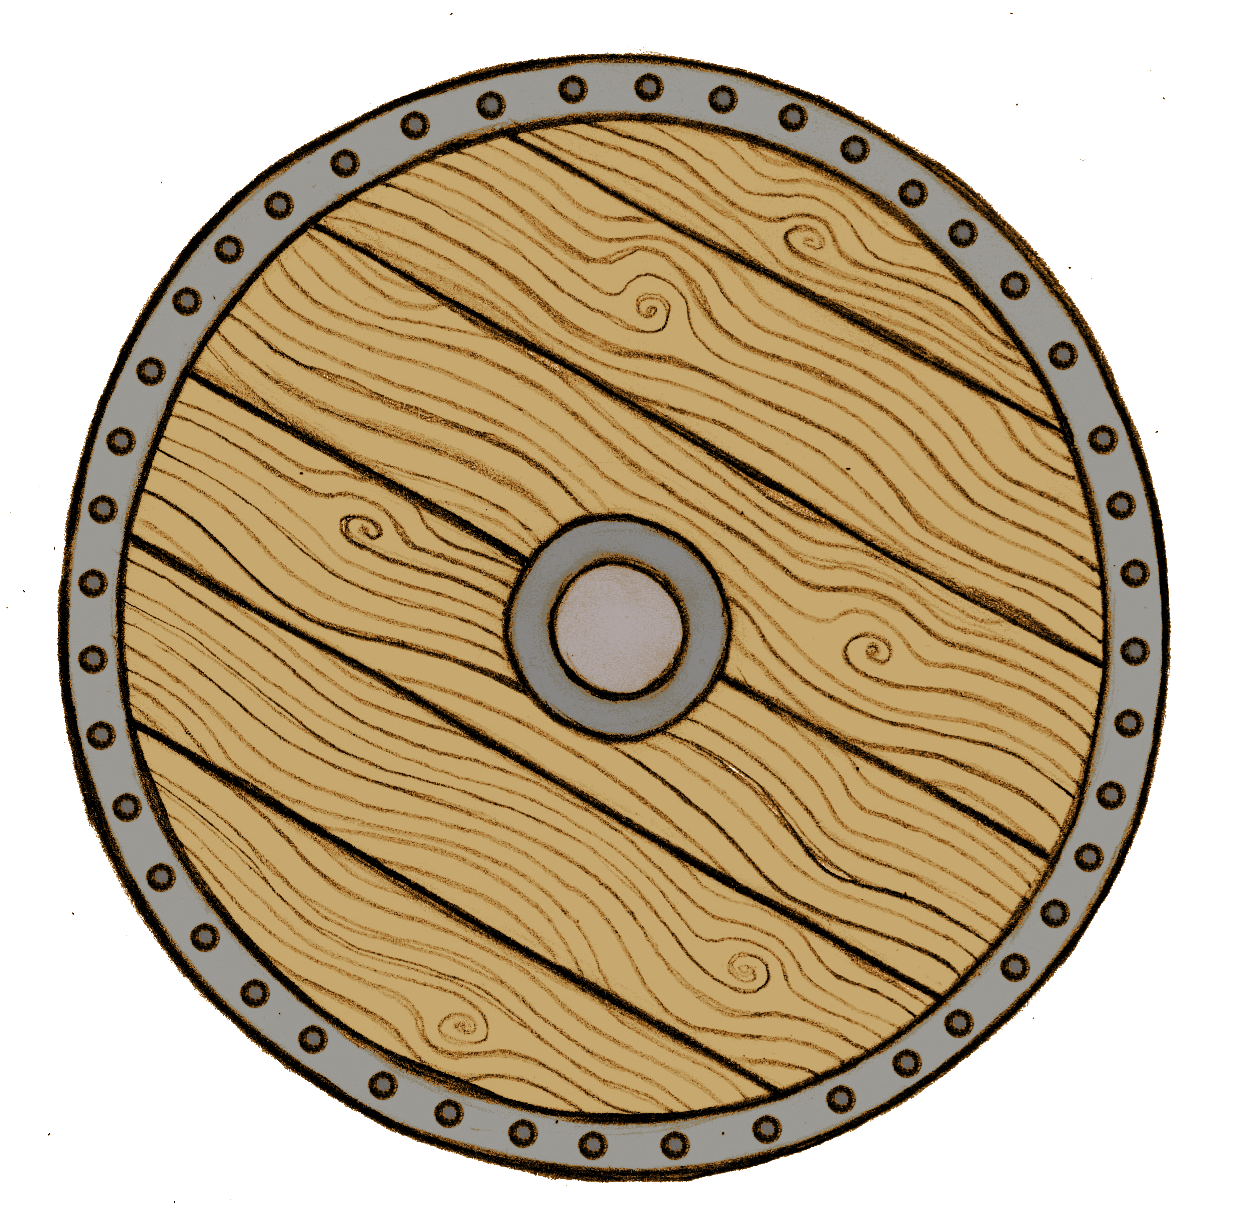
\includegraphics[height=30mm]{img/Jorvik/objects/shields/plain shield}}\\
		Plain Shield & \\ 
		\textbf{Price:} & \\
		35.29 Silver & \\ 
		\textbf{Description:} & \\
		\multicolumn{2}{p{12cm}}{Viking shields could be made from a range of woods including fir, pine, willow and linden. Many were covered in leather, linen and wool to add extra strength against weapons.}\\
		\bottomrule
	\end{tabular}
\end{table}